\documentclass[10pt,twocolumn,a4paper]{article}
\usepackage[utf8]{inputenc}
\usepackage{fontenc}
\usepackage[french]{babel}
\usepackage[top=1cm, bottom=1cm, left=1cm, right=1cm]{geometry}
\usepackage{graphicx}
\usepackage{lmodern}
\usepackage{amsmath}
\usepackage{amssymb}
\usepackage{mathrsfs}
\usepackage{multirow}
\usepackage{schemabloc}

\title{Théorie des circuits}
\date{\today}
\author{Guilhem Saurel}

\begin{document}
\maketitle
Norton/Thévenin : G/R src. ind. off \& J/V en CO/CC

$Z_{th}$ on ajoute soit une source de courant et on regarde la tension, soit une source de tension et on regarde le courant

$s(t)= \cfrac{a_0}{2} + \sum_{n=1}^{\infty}{\left( a_n \cos\left(n\omega t\right) + b_n \sin\left(n \omega t \right) \right)}$

$a_n = \cfrac{2}{T} \int \limits_{-T/2}^{T/2}{s(t)\cos\left(n\omega t\right) dt}$

$b_n = \cfrac{2}{T} \int \limits_{-T/2}^{T/2}{s(t)\sin\left(n\omega t\right) dt}$

$D_n = \sqrt{a_n^2+b_n^2}$

$\tan\varphi_n = - \cfrac{b_n}{a_n}$

$F_{eff} = \sqrt{D_0^2 + \cfrac{1}{2}\sum_{n=1}^{\infty}{D_n^2}}$

facteur de forme : $F = \cfrac{F_{eff}}{F{moy}}$

taux d'ondulation : $\beta = \cfrac{\sqrt{\cfrac{1}{2}\sum_{n=1}^{\infty}{D_n^2}}}{D_0}$

taux de distorsion harmonique : $\tau = \cfrac{\sqrt{\cfrac{1}{2}\sum_{n=2}^{\infty}{D_n^2}}}{D_1}$

$\begin{bmatrix}V_1 \\ I_1\end{bmatrix} = \begin{bmatrix}A&B\\C&D \end{bmatrix}\begin{bmatrix}V_2\\-I_2 \end{bmatrix}$

$\begin{bmatrix}V_1\\I_2 \end{bmatrix} =\begin{bmatrix}h_{11}&h{12}\\h{21}&h{22} \end{bmatrix}\begin{bmatrix}I_1\\V_2 \end{bmatrix} $

$\begin{bmatrix}I_1\\V_2 \end{bmatrix} =\begin{bmatrix}g_{11}&g{12}\\g{21}&g{22} \end{bmatrix}\begin{bmatrix}V_1\\I_2 \end{bmatrix} $

$Z_e = Z_{11} - \cfrac{Z_{12}Z_{21}}{Z_{22} + Z_u}$

$Z_s = Z_{22} - \cfrac{Z_{12}Z_{21}}{Z_{11} + Z_g}$

quadripoles chaine : produit des A

quadripoles série : somme des Z

quadripoles parallèle : somme des Y

$T_v = \cfrac{Z_u Z_{21}}{Z_e(Z_{22}+Z_u)}$

$T_i = \cfrac{Z_21}{Z_{22}+Z_u}$

$f(t)u(t) \rightarrow F(p)$

$\delta (t) \rightarrow 1 $

$u(t) \rightarrow 1/p$

$e^{-at}u(t) \rightarrow \cfrac{1}{p+a}$

$t^nu(t) \rightarrow \cfrac{n!}{p^{n+1}}$

$\cos(\omega t) u(t) \rightarrow \cfrac{p}{p^2 + \omega^2}$

$\sin(\omega t) u(t) \rightarrow \cfrac{\omega}{p^2 + \omega^2}$

$A\cos(\omega t + \varphi) \rightarrow A \cfrac{p\cos \varphi - \omega\sin\varphi}{p^2 + \omega^2}$

$A\sin(\omega t + \varphi) \rightarrow A \cfrac{p\sin \varphi + \omega\cos\varphi}{p^2 + \omega^2}$

$e^{-at}\cos(\omega t) u(t) \rightarrow \cfrac{p+a}{p^2 + \omega^2}$

$e^{-at}\sin(\omega t) u(t) \rightarrow \cfrac{\omega}{(p+a)^2 + \omega^2}$

$t^ne^{-at}u(t) \rightarrow \cfrac{n!}{(p+a)^{n+1}}$

$\cfrac{1}{\sqrt{\pi t}} \rightarrow \cfrac{1}{\sqrt{p}}$

$\cfrac{df(t)}{dt}u(t) \rightarrow pF(p) - f(0^-)$

$\cfrac{d^2f(t)}{dt^2} u(t) \rightarrow p^2F(p) - pf(0^-) - f(0^-)$

$\int \limits_{0}^{t}{f(t)dt} \rightarrow \cfrac{F(p)}{p}$

$e^{-at}f(t)u(t) \rightarrow F(p+a)$

$f(t-t_0)u(t-t_0) \rightarrow F(p)e^{-t_0p}$

$f(at)u(t) \rightarrow \cfrac{1}{a}F\left(\cfrac{p}{a}\right)$

$-tf(t)u(t) \rightarrow \cfrac{dF(p)}{dp} $

$\cfrac{f(t)}{t} u(t) \rightarrow \int \limits_{p}^{\infty}{F(p)dp} $

$ \lim \limits_{p \to 0} pF(p) = \lim \limits_{p \to \infty} f(t)$


$ \lim \limits_{p \to \infty} pF(p) = \lim \limits_{p \to 0^+} f(t)$

$(f(t)\ast g(t)) u(t) \rightarrow F(p)G(p)$

$f(t)g(t) u(t) \rightarrow F(p)\ast G(p)$

$F(p) = \cfrac{A}{p-a} + \cfrac{B}{p-b} + \cfrac{C}{p-c} \rightarrow f(t) = Ae^{at}+Be^{bt}+Ce^{ct}$

energie : $E = \int \limits_{-\infty}^{+\infty} x^2(t)dt$


\newpage

\includegraphics[width=16cm]{tableau.jpg}
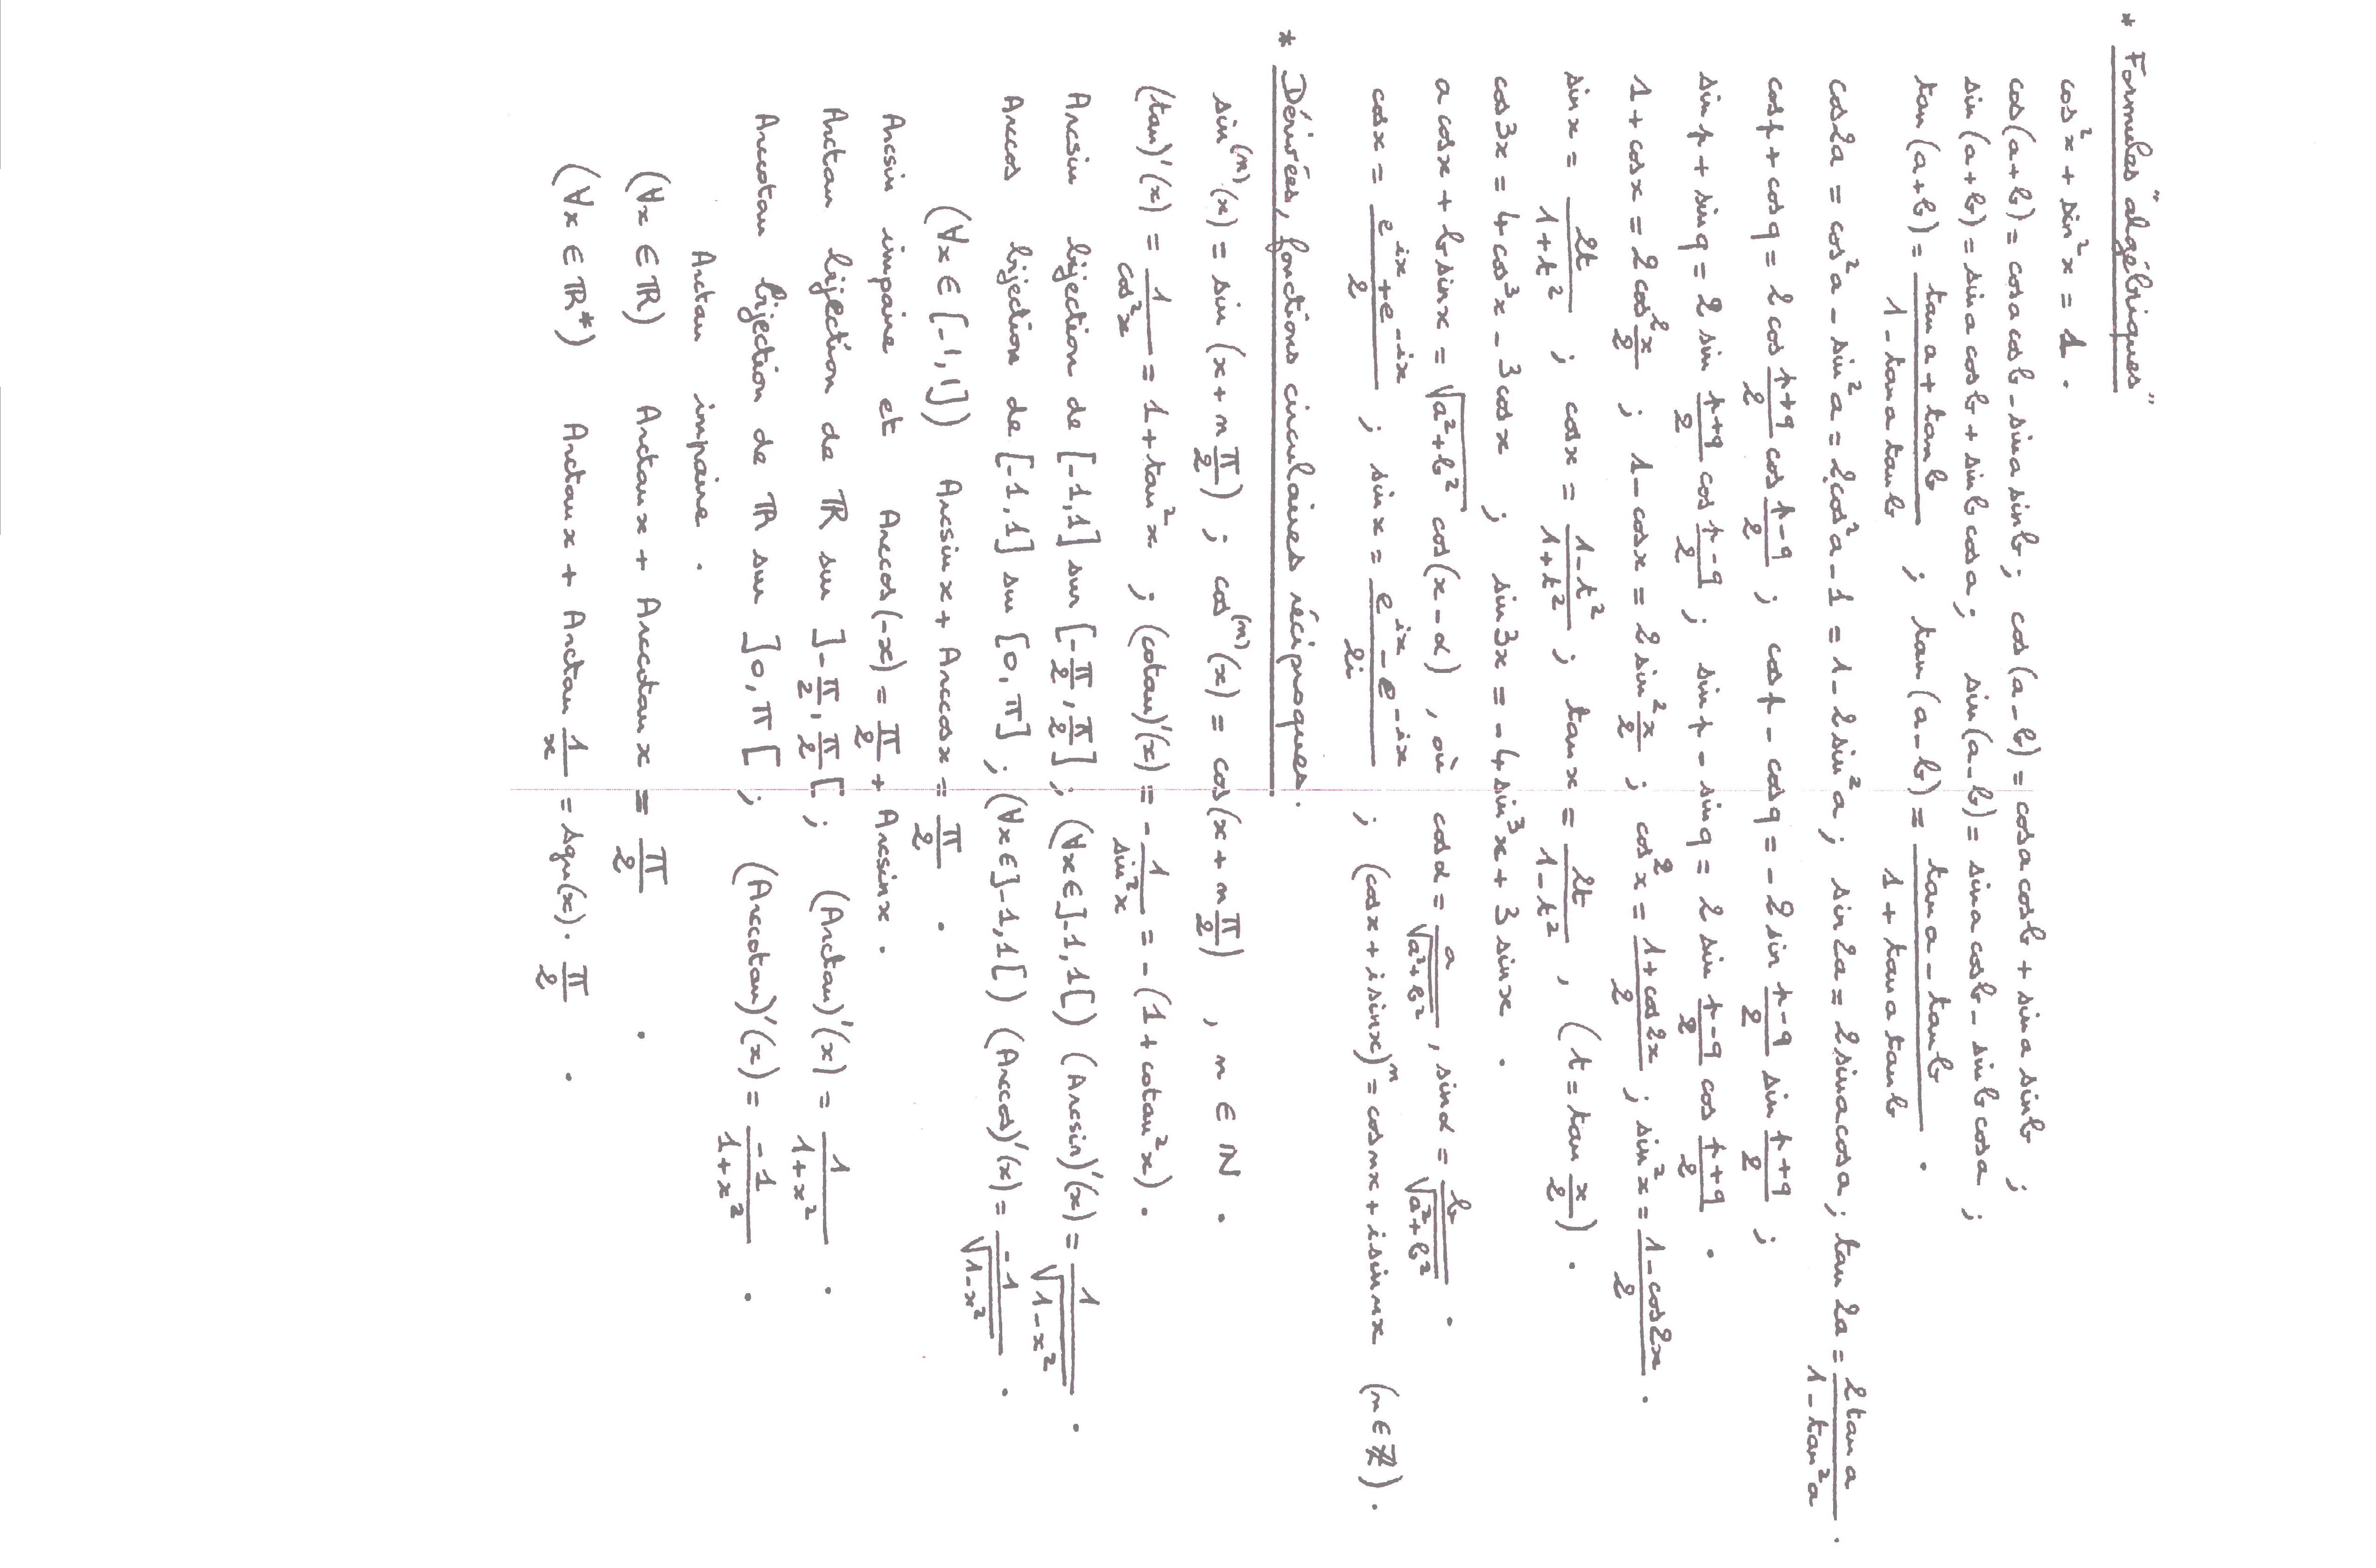
\includegraphics[width=16cm]{../trigo/trigo1.jpg}



\end{document}

